\documentclass[a4paper]{book}
\usepackage{a4wide}
\usepackage{makeidx}
\usepackage{graphicx}
\usepackage{multicol}
\usepackage{float}
\usepackage{listings}
\usepackage{color}
\usepackage{textcomp}
\usepackage{alltt}
\usepackage{times}
\usepackage{ifpdf}
\ifpdf
\usepackage[pdftex,
            pagebackref=true,
            colorlinks=true,
            linkcolor=blue,
            unicode
           ]{hyperref}
\else
\usepackage[ps2pdf,
            pagebackref=true,
            colorlinks=true,
            linkcolor=blue,
            unicode
           ]{hyperref}
\usepackage{pspicture}
\fi
\usepackage[utf8]{inputenc}
\usepackage{doxygen}
\lstset{language=C++,inputencoding=utf8,basicstyle=\footnotesize,breaklines=true,breakatwhitespace=true,tabsize=8,numbers=left }
\makeindex
\setcounter{tocdepth}{3}
\renewcommand{\footrulewidth}{0.4pt}
\begin{document}
\hypersetup{pageanchor=false}
\begin{titlepage}
\vspace*{7cm}
\begin{center}
{\Large MediGL }\\
\vspace*{1cm}
{\large Generated by Doxygen 1.6.3}\\
\vspace*{0.5cm}
{\small Thu Jul 1 20:13:42 2010}\\
\end{center}
\end{titlepage}
\clearemptydoublepage
\pagenumbering{roman}
\tableofcontents
\clearemptydoublepage
\pagenumbering{arabic}
\hypersetup{pageanchor=true}
\chapter{Class Index}
\section{Class List}
Here are the classes, structs, unions and interfaces with brief descriptions:\begin{DoxyCompactList}
\item\contentsline{section}{\hyperlink{struct_c4_u_b_v3_f}{C4UBV3F} }{\pageref{struct_c4_u_b_v3_f}}{}
\item\contentsline{section}{\hyperlink{class_d_i_c_o_m_image_file}{DICOMImageFile} }{\pageref{class_d_i_c_o_m_image_file}}{}
\item\contentsline{section}{\hyperlink{class_fast_image}{FastImage} }{\pageref{class_fast_image}}{}
\item\contentsline{section}{\hyperlink{class_g_l_widget}{GLWidget} }{\pageref{class_g_l_widget}}{}
\item\contentsline{section}{\hyperlink{class_medi_dialog}{MediDialog} }{\pageref{class_medi_dialog}}{}
\end{DoxyCompactList}

\chapter{Class Documentation}
\hypertarget{struct_c4_u_b_v3_f}{
\section{C4UBV3F Struct Reference}
\label{struct_c4_u_b_v3_f}\index{C4UBV3F@{C4UBV3F}}
}
\subsection*{Public Attributes}
\begin{DoxyCompactItemize}
\item 
\hypertarget{struct_c4_u_b_v3_f_af6a7e78a2f2e724b7755d03d5644b0dc}{
unsigned char {\bfseries color} \mbox{[}4\mbox{]}}
\label{struct_c4_u_b_v3_f_af6a7e78a2f2e724b7755d03d5644b0dc}

\item 
\hypertarget{struct_c4_u_b_v3_f_ae82b7ce1479a879d5bac242d64bc6c3d}{
float {\bfseries vcoords} \mbox{[}3\mbox{]}}
\label{struct_c4_u_b_v3_f_ae82b7ce1479a879d5bac242d64bc6c3d}

\end{DoxyCompactItemize}


The documentation for this struct was generated from the following file:\begin{DoxyCompactItemize}
\item 
glwidget.cpp\end{DoxyCompactItemize}

\hypertarget{class_d_i_c_o_m_image_file}{
\section{DICOMImageFile Class Reference}
\label{class_d_i_c_o_m_image_file}\index{DICOMImageFile@{DICOMImageFile}}
}


{\ttfamily \#include $<$dicomimagefile.h$>$}

\subsection*{Public Member Functions}
\begin{DoxyCompactItemize}
\item 
\hyperlink{class_d_i_c_o_m_image_file_ae4778b6e6ed2c36f47fe3e785b55bb2e}{DICOMImageFile} (string filename)
\item 
\hyperlink{class_fast_image}{FastImage} $\ast$ \hyperlink{class_d_i_c_o_m_image_file_aac6cfe1b8babedd17543fd3a8971f86b}{getFastImage} (uint frame, bool contrastExtension, bool enableWindow=false, double windowCenter=0.0, double windowWidth=0.0)
\item 
uint \hyperlink{class_d_i_c_o_m_image_file_a4eb4186345395c61c7964e588a08e057}{getWidth} ()
\item 
uint \hyperlink{class_d_i_c_o_m_image_file_abebf0dfb003c75c06c3955e65dd5b9a6}{getHeight} ()
\item 
uint \hyperlink{class_d_i_c_o_m_image_file_aec56b3e9d86b2af4206e38406714941f}{getFrameCount} ()
\item 
\hyperlink{class_d_i_c_o_m_image_file_af210a193559ee3287aa1f9c4bf13d3ab}{$\sim$DICOMImageFile} ()
\end{DoxyCompactItemize}
\subsection*{Protected Attributes}
\begin{DoxyCompactItemize}
\item 
\hypertarget{class_d_i_c_o_m_image_file_ac8700ef1684e13d0d0fe01e603294293}{
DicomImage $\ast$ {\bfseries image}}
\label{class_d_i_c_o_m_image_file_ac8700ef1684e13d0d0fe01e603294293}

\item 
\hypertarget{class_d_i_c_o_m_image_file_af62a20b7e1e3a7a33ddc848b429b64f8}{
uint {\bfseries width}}
\label{class_d_i_c_o_m_image_file_af62a20b7e1e3a7a33ddc848b429b64f8}

\item 
\hypertarget{class_d_i_c_o_m_image_file_ae751485a997fefa6136cfe40255a38c6}{
uint {\bfseries height}}
\label{class_d_i_c_o_m_image_file_ae751485a997fefa6136cfe40255a38c6}

\item 
\hypertarget{class_d_i_c_o_m_image_file_a445cb53cda79233bb1815a96bb3fa97b}{
uint {\bfseries frameCount}}
\label{class_d_i_c_o_m_image_file_a445cb53cda79233bb1815a96bb3fa97b}

\end{DoxyCompactItemize}


\subsection{Detailed Description}
Wrapper class for easy use of the DICOM file format (DICOM images only) Uses the DCMTK library to process DICOM files. 

\subsection{Constructor \& Destructor Documentation}
\hypertarget{class_d_i_c_o_m_image_file_ae4778b6e6ed2c36f47fe3e785b55bb2e}{
\index{DICOMImageFile@{DICOMImageFile}!DICOMImageFile@{DICOMImageFile}}
\index{DICOMImageFile@{DICOMImageFile}!DICOMImageFile@{DICOMImageFile}}
\subsubsection[{DICOMImageFile}]{\setlength{\rightskip}{0pt plus 5cm}DICOMImageFile::DICOMImageFile (
\begin{DoxyParamCaption}
\item[{string}]{ filename}
\end{DoxyParamCaption}
)}}
\label{class_d_i_c_o_m_image_file_ae4778b6e6ed2c36f47fe3e785b55bb2e}
Constructs a new \hyperlink{class_d_i_c_o_m_image_file}{DICOMImageFile} instance by a given filename Occuring errors are logged to cerr. \hypertarget{class_d_i_c_o_m_image_file_af210a193559ee3287aa1f9c4bf13d3ab}{
\index{DICOMImageFile@{DICOMImageFile}!$\sim$DICOMImageFile@{$\sim$DICOMImageFile}}
\index{$\sim$DICOMImageFile@{$\sim$DICOMImageFile}!DICOMImageFile@{DICOMImageFile}}
\subsubsection[{$\sim$DICOMImageFile}]{\setlength{\rightskip}{0pt plus 5cm}DICOMImageFile::$\sim$DICOMImageFile (
\begin{DoxyParamCaption}
{}
\end{DoxyParamCaption}
)}}
\label{class_d_i_c_o_m_image_file_af210a193559ee3287aa1f9c4bf13d3ab}
Releases all resources acquired by this \hyperlink{class_d_i_c_o_m_image_file}{DICOMImageFile} instance 

\subsection{Member Function Documentation}
\hypertarget{class_d_i_c_o_m_image_file_aac6cfe1b8babedd17543fd3a8971f86b}{
\index{DICOMImageFile@{DICOMImageFile}!getFastImage@{getFastImage}}
\index{getFastImage@{getFastImage}!DICOMImageFile@{DICOMImageFile}}
\subsubsection[{getFastImage}]{\setlength{\rightskip}{0pt plus 5cm}{\bf FastImage} $\ast$ DICOMImageFile::getFastImage (
\begin{DoxyParamCaption}
\item[{uint}]{ frame, }
\item[{bool}]{ contrastExtension, }
\item[{bool}]{ enableWindow = {\ttfamily false}, }
\item[{double}]{ windowCenter = {\ttfamily 0.0}, }
\item[{double}]{ windowWidth = {\ttfamily 0.0}}
\end{DoxyParamCaption}
)}}
\label{class_d_i_c_o_m_image_file_aac6cfe1b8babedd17543fd3a8971f86b}
Constructs a new \hyperlink{class_fast_image}{FastImage} instance with the contents of a specific file this DICOM image file 
\begin{DoxyParams}{Parameters}
\item[{\em frame}]The number of the frame (beginning with 0) to use \item[{\em contrastExtension}]Whether to spread the values in the resulting grayscale image to the full available range. Not recommendened when using a Hounsfield window \item[{\em enableWindow}]Whether to use a Hounsfield window \item[{\em windowCenter}]The center of the Hounsfield window, if enabled \item[{\em windowWidth}]The width of the Hounsfield window, if enabled \end{DoxyParams}


Here is the call graph for this function:
\nopagebreak
\begin{figure}[H]
\begin{center}
\leavevmode
\includegraphics[width=400pt]{class_d_i_c_o_m_image_file_aac6cfe1b8babedd17543fd3a8971f86b_cgraph}
\end{center}
\end{figure}


\hypertarget{class_d_i_c_o_m_image_file_aec56b3e9d86b2af4206e38406714941f}{
\index{DICOMImageFile@{DICOMImageFile}!getFrameCount@{getFrameCount}}
\index{getFrameCount@{getFrameCount}!DICOMImageFile@{DICOMImageFile}}
\subsubsection[{getFrameCount}]{\setlength{\rightskip}{0pt plus 5cm}uint DICOMImageFile::getFrameCount (
\begin{DoxyParamCaption}
{}
\end{DoxyParamCaption}
)\hspace{0.3cm}{\ttfamily  \mbox{[}inline\mbox{]}}}}
\label{class_d_i_c_o_m_image_file_aec56b3e9d86b2af4206e38406714941f}
\begin{DoxyReturn}{Returns}
The frame count of this image 
\end{DoxyReturn}
\hypertarget{class_d_i_c_o_m_image_file_abebf0dfb003c75c06c3955e65dd5b9a6}{
\index{DICOMImageFile@{DICOMImageFile}!getHeight@{getHeight}}
\index{getHeight@{getHeight}!DICOMImageFile@{DICOMImageFile}}
\subsubsection[{getHeight}]{\setlength{\rightskip}{0pt plus 5cm}uint DICOMImageFile::getHeight (
\begin{DoxyParamCaption}
{}
\end{DoxyParamCaption}
)\hspace{0.3cm}{\ttfamily  \mbox{[}inline\mbox{]}}}}
\label{class_d_i_c_o_m_image_file_abebf0dfb003c75c06c3955e65dd5b9a6}
\begin{DoxyReturn}{Returns}
The height of this image 
\end{DoxyReturn}
\hypertarget{class_d_i_c_o_m_image_file_a4eb4186345395c61c7964e588a08e057}{
\index{DICOMImageFile@{DICOMImageFile}!getWidth@{getWidth}}
\index{getWidth@{getWidth}!DICOMImageFile@{DICOMImageFile}}
\subsubsection[{getWidth}]{\setlength{\rightskip}{0pt plus 5cm}uint DICOMImageFile::getWidth (
\begin{DoxyParamCaption}
{}
\end{DoxyParamCaption}
)\hspace{0.3cm}{\ttfamily  \mbox{[}inline\mbox{]}}}}
\label{class_d_i_c_o_m_image_file_a4eb4186345395c61c7964e588a08e057}
\begin{DoxyReturn}{Returns}
The width of this image 
\end{DoxyReturn}


The documentation for this class was generated from the following files:\begin{DoxyCompactItemize}
\item 
dicomimagefile.h\item 
dicomimagefile.cpp\end{DoxyCompactItemize}

\hypertarget{class_fast_image}{
\section{FastImage Class Reference}
\label{class_fast_image}\index{FastImage@{FastImage}}
}


{\ttfamily \#include $<$fastimage.h$>$}

\subsection*{Public Member Functions}
\begin{DoxyCompactItemize}
\item 
\hyperlink{class_fast_image_a1ee91a3ac8ddcdfed90e9906bb3f0681}{FastImage} (QImage $\ast$img, bool enableGrayCache=true)
\item 
\hyperlink{class_fast_image_ab9530428f52635d4f87d9b1cc33e10cd}{FastImage} (uint width, uint height, bool enableGrayCache=true)
\item 
\hyperlink{class_fast_image_ae2937f18d549ffc788abaa1a5bf6f492}{$\sim$FastImage} ()
\item 
uint32\_\-t \hyperlink{class_fast_image_a09e6df8ae76ddffb813048157f887ee6}{getRgba} (uint x, uint y)
\item 
char \hyperlink{class_fast_image_a7da37f6c5c99feea80c6a699c7b51bd8}{getGray} (uint x, uint y)
\item 
double \hyperlink{class_fast_image_a6975ad540e89b98fda1b7a3bd3f812ea}{getGray32bit} (uint x, uint y)
\item 
void \hyperlink{class_fast_image_a647ac3b76f0198da77cd2e7afa46e1c4}{setPixel} (uint x, uint y, uint32\_\-t val)
\item 
void \hyperlink{class_fast_image_a1e0ef4ac5b61cc6d96c9cd9c4bada344}{setGrayPixel} (uint x, uint y, unsigned char val)
\item 
void \hyperlink{class_fast_image_a018ae53445320129fa129b80e805842c}{setGrayPixel} (uint x, uint y, uint32\_\-t val)
\item 
void \hyperlink{class_fast_image_adcf6d77e79c1f75f2420c6db0d96951d}{spreadContrast} ()
\item 
uint \hyperlink{class_fast_image_a94290d65ff847f0a7e56ac8050133313}{getWidth} ()
\item 
uint \hyperlink{class_fast_image_a1b90d63510575306ce345e393574d85c}{getHeight} ()
\end{DoxyCompactItemize}
\subsection*{Protected Attributes}
\begin{DoxyCompactItemize}
\item 
\hypertarget{class_fast_image_ae8bc71fe6069de24a12214fc3828ca6d}{
uint {\bfseries width}}
\label{class_fast_image_ae8bc71fe6069de24a12214fc3828ca6d}

\item 
\hypertarget{class_fast_image_aca3f4d119be3052564a7b95645e416ae}{
uint {\bfseries height}}
\label{class_fast_image_aca3f4d119be3052564a7b95645e416ae}

\item 
\hypertarget{class_fast_image_aced6ae3b9e826ed23b1e35e0556b9e0e}{
bool {\bfseries grayCacheEnabled}}
\label{class_fast_image_aced6ae3b9e826ed23b1e35e0556b9e0e}

\item 
\hypertarget{class_fast_image_a1694943fbf3cd250f629c70c07d89e6e}{
uint32\_\-t $\ast$ {\bfseries colorData}}
\label{class_fast_image_a1694943fbf3cd250f629c70c07d89e6e}

\item 
\hypertarget{class_fast_image_ab0eae6bc0937543738d336a9b4f1a68c}{
double $\ast$ {\bfseries grayData}}
\label{class_fast_image_ab0eae6bc0937543738d336a9b4f1a68c}

\end{DoxyCompactItemize}


\subsection{Detailed Description}
Image wrapper class internally using arrays for fast read access Optimized for read access Compiling with -\/fno-\/strict-\/aliasing should make this class faster

One instance of this class represents exactly one image. \hyperlink{class_fast_image}{FastImage} can build a gray cache to be able to serve \hyperlink{class_fast_image_a7da37f6c5c99feea80c6a699c7b51bd8}{getGray()} requests very fast. This feature is enabled by default but can be disabled. Users are not encouraged to change the data using setPixel(...).

\hyperlink{class_fast_image}{FastImage} internally stores the data using 64 bit floating point numbers

\hyperlink{class_fast_image}{FastImage} is optimized to process grayscale images -\/ some functions only work on grayscale images

The purpose of this class is to have a fast, scalable abstraction layer between MediGL input data and OpenGL in order to be able to support a variety of image formats. 

\subsection{Constructor \& Destructor Documentation}
\hypertarget{class_fast_image_a1ee91a3ac8ddcdfed90e9906bb3f0681}{
\index{FastImage@{FastImage}!FastImage@{FastImage}}
\index{FastImage@{FastImage}!FastImage@{FastImage}}
\subsubsection[{FastImage}]{\setlength{\rightskip}{0pt plus 5cm}FastImage::FastImage (QImage $\ast$ {\em img}, \/  bool {\em enableGrayCache} = {\ttfamily true})}}
\label{class_fast_image_a1ee91a3ac8ddcdfed90e9906bb3f0681}
Creates a new \hyperlink{class_fast_image}{FastImage} instance from a QImage. Uses the data from the QImage instance to fill the cache 
\begin{DoxyParams}{Parameters}
\item[{\em img}]The image to process \item[{\em enableGrayCache}]Whether to enable a separate gray cache \end{DoxyParams}
\hypertarget{class_fast_image_ab9530428f52635d4f87d9b1cc33e10cd}{
\index{FastImage@{FastImage}!FastImage@{FastImage}}
\index{FastImage@{FastImage}!FastImage@{FastImage}}
\subsubsection[{FastImage}]{\setlength{\rightskip}{0pt plus 5cm}FastImage::FastImage (uint {\em width}, \/  uint {\em height}, \/  bool {\em enableGrayCache} = {\ttfamily true})}}
\label{class_fast_image_ab9530428f52635d4f87d9b1cc33e10cd}
Creates a new \hyperlink{class_fast_image}{FastImage} instance with given width and height but without any content. Use setPixel(...) to set the pixels 
\begin{DoxyParams}{Parameters}
\item[{\em width}]The widi of the new image \item[{\em height}]The height of the new image \item[{\em enableGrayCache}]Whether to enable a separate gray cache \end{DoxyParams}
\hypertarget{class_fast_image_ae2937f18d549ffc788abaa1a5bf6f492}{
\index{FastImage@{FastImage}!$\sim$FastImage@{$\sim$FastImage}}
\index{$\sim$FastImage@{$\sim$FastImage}!FastImage@{FastImage}}
\subsubsection[{$\sim$FastImage}]{\setlength{\rightskip}{0pt plus 5cm}FastImage::$\sim$FastImage ()}}
\label{class_fast_image_ae2937f18d549ffc788abaa1a5bf6f492}
Releases all memory occupied by this \hyperlink{class_fast_image}{FastImage} instance 

\subsection{Member Function Documentation}
\hypertarget{class_fast_image_a7da37f6c5c99feea80c6a699c7b51bd8}{
\index{FastImage@{FastImage}!getGray@{getGray}}
\index{getGray@{getGray}!FastImage@{FastImage}}
\subsubsection[{getGray}]{\setlength{\rightskip}{0pt plus 5cm}char FastImage::getGray (uint {\em x}, \/  uint {\em y})}}
\label{class_fast_image_a7da37f6c5c99feea80c6a699c7b51bd8}
Gets the gray value (8 bit) for specific x and y pixel coordinates. The request is served from the gray cache if it has been enabled for this instance \hypertarget{class_fast_image_a6975ad540e89b98fda1b7a3bd3f812ea}{
\index{FastImage@{FastImage}!getGray32bit@{getGray32bit}}
\index{getGray32bit@{getGray32bit}!FastImage@{FastImage}}
\subsubsection[{getGray32bit}]{\setlength{\rightskip}{0pt plus 5cm}double FastImage::getGray32bit (uint {\em x}, \/  uint {\em y})}}
\label{class_fast_image_a6975ad540e89b98fda1b7a3bd3f812ea}
Gets the gray value (8 bit) for specific x and y pixel coordinates. The request is served from the gray cache if it has been enabled for this instance \hypertarget{class_fast_image_a1b90d63510575306ce345e393574d85c}{
\index{FastImage@{FastImage}!getHeight@{getHeight}}
\index{getHeight@{getHeight}!FastImage@{FastImage}}
\subsubsection[{getHeight}]{\setlength{\rightskip}{0pt plus 5cm}uint FastImage::getHeight ()\hspace{0.3cm}{\ttfamily  \mbox{[}inline\mbox{]}}}}
\label{class_fast_image_a1b90d63510575306ce345e393574d85c}
\begin{DoxyReturn}{Returns}
The height of this image 
\end{DoxyReturn}
\hypertarget{class_fast_image_a09e6df8ae76ddffb813048157f887ee6}{
\index{FastImage@{FastImage}!getRgba@{getRgba}}
\index{getRgba@{getRgba}!FastImage@{FastImage}}
\subsubsection[{getRgba}]{\setlength{\rightskip}{0pt plus 5cm}uint32\_\-t FastImage::getRgba (uint {\em x}, \/  uint {\em y})}}
\label{class_fast_image_a09e6df8ae76ddffb813048157f887ee6}
Gets the RGBA value for a specific pixel in this \hyperlink{class_fast_image}{FastImage} instance.

This function does NOT check if the x and y parameters are in the bounds of this \hyperlink{class_fast_image}{FastImage} instance for sake of performance \hypertarget{class_fast_image_a94290d65ff847f0a7e56ac8050133313}{
\index{FastImage@{FastImage}!getWidth@{getWidth}}
\index{getWidth@{getWidth}!FastImage@{FastImage}}
\subsubsection[{getWidth}]{\setlength{\rightskip}{0pt plus 5cm}uint FastImage::getWidth ()\hspace{0.3cm}{\ttfamily  \mbox{[}inline\mbox{]}}}}
\label{class_fast_image_a94290d65ff847f0a7e56ac8050133313}
\begin{DoxyReturn}{Returns}
The width of this image 
\end{DoxyReturn}
\hypertarget{class_fast_image_a018ae53445320129fa129b80e805842c}{
\index{FastImage@{FastImage}!setGrayPixel@{setGrayPixel}}
\index{setGrayPixel@{setGrayPixel}!FastImage@{FastImage}}
\subsubsection[{setGrayPixel}]{\setlength{\rightskip}{0pt plus 5cm}void FastImage::setGrayPixel (uint {\em x}, \/  uint {\em y}, \/  uint32\_\-t {\em val})}}
\label{class_fast_image_a018ae53445320129fa129b80e805842c}
Sets a pixel to a specific gray value. The color buffer is not affected. 
\begin{DoxyParams}{Parameters}
\item[{\em x}]The x coordinate of the pixel to set \item[{\em y}]The x coordinate of the pixel to set \item[{\em val}]The 32-\/bit grayscale value to set the pixel to \end{DoxyParams}
\hypertarget{class_fast_image_a1e0ef4ac5b61cc6d96c9cd9c4bada344}{
\index{FastImage@{FastImage}!setGrayPixel@{setGrayPixel}}
\index{setGrayPixel@{setGrayPixel}!FastImage@{FastImage}}
\subsubsection[{setGrayPixel}]{\setlength{\rightskip}{0pt plus 5cm}void FastImage::setGrayPixel (uint {\em x}, \/  uint {\em y}, \/  unsigned char {\em val})}}
\label{class_fast_image_a1e0ef4ac5b61cc6d96c9cd9c4bada344}
Sets a pixel to a specific gray value. The color buffer is not affected. 
\begin{DoxyParams}{Parameters}
\item[{\em x}]The x coordinate of the pixel to set \item[{\em y}]The x coordinate of the pixel to set \item[{\em val}]The grayscale value to set the pixel to \end{DoxyParams}


Here is the caller graph for this function:\nopagebreak
\begin{figure}[H]
\begin{center}
\leavevmode
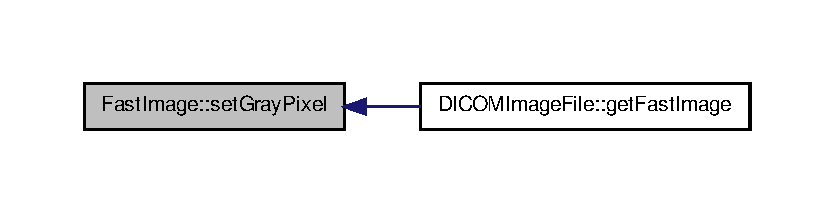
\includegraphics[width=182pt]{class_fast_image_a1e0ef4ac5b61cc6d96c9cd9c4bada344_icgraph}
\end{center}
\end{figure}


\hypertarget{class_fast_image_a647ac3b76f0198da77cd2e7afa46e1c4}{
\index{FastImage@{FastImage}!setPixel@{setPixel}}
\index{setPixel@{setPixel}!FastImage@{FastImage}}
\subsubsection[{setPixel}]{\setlength{\rightskip}{0pt plus 5cm}void FastImage::setPixel (uint {\em x}, \/  uint {\em y}, \/  uint32\_\-t {\em val})}}
\label{class_fast_image_a647ac3b76f0198da77cd2e7afa46e1c4}
Sets a pixel in this \hyperlink{class_fast_image}{FastImage} instance to a specific value and updates the gray cache if it is enabled 
\begin{DoxyParams}{Parameters}
\item[{\em x}]The x coordinate of the pixel to set \item[{\em y}]The x coordinate of the pixel to set \item[{\em val}]The RGBA value to set the pixel to \end{DoxyParams}
\hypertarget{class_fast_image_adcf6d77e79c1f75f2420c6db0d96951d}{
\index{FastImage@{FastImage}!spreadContrast@{spreadContrast}}
\index{spreadContrast@{spreadContrast}!FastImage@{FastImage}}
\subsubsection[{spreadContrast}]{\setlength{\rightskip}{0pt plus 5cm}void FastImage::spreadContrast ()}}
\label{class_fast_image_adcf6d77e79c1f75f2420c6db0d96951d}
Performs a constrast spreading on the gray data of this \hyperlink{class_fast_image}{FastImage}.

The algorithm used has a linear complexity

Note: The color data is not affected! 

Here is the caller graph for this function:\nopagebreak
\begin{figure}[H]
\begin{center}
\leavevmode
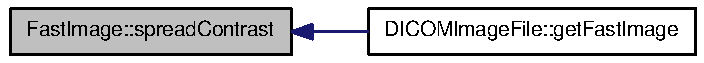
\includegraphics[width=187pt]{class_fast_image_adcf6d77e79c1f75f2420c6db0d96951d_icgraph}
\end{center}
\end{figure}




The documentation for this class was generated from the following files:\begin{DoxyCompactItemize}
\item 
fastimage.h\item 
fastimage.cpp\end{DoxyCompactItemize}

\hypertarget{class_g_l_widget}{
\section{GLWidget Class Reference}
\label{class_g_l_widget}\index{GLWidget@{GLWidget}}
}


{\ttfamily \#include $<$glwidget.h$>$}

\subsection*{Public Slots}
\begin{DoxyCompactItemize}
\item 
\hypertarget{class_g_l_widget_a7083404e9ab8feffb2c486f7c15308ce}{
void {\bfseries setXRotation} (int angle)}
\label{class_g_l_widget_a7083404e9ab8feffb2c486f7c15308ce}

\item 
\hypertarget{class_g_l_widget_a29012eba3cb4201f78807066f2c9dcd4}{
void {\bfseries setYRotation} (int angle)}
\label{class_g_l_widget_a29012eba3cb4201f78807066f2c9dcd4}

\item 
\hypertarget{class_g_l_widget_a6f6b4fbbcc566d999db7e53aadeba889}{
void {\bfseries setZRotation} (int angle)}
\label{class_g_l_widget_a6f6b4fbbcc566d999db7e53aadeba889}

\end{DoxyCompactItemize}
\subsection*{Signals}
\begin{DoxyCompactItemize}
\item 
\hypertarget{class_g_l_widget_a3a557b9cd96f7b89661ceaa567c91640}{
void {\bfseries xRotationChanged} (int angle)}
\label{class_g_l_widget_a3a557b9cd96f7b89661ceaa567c91640}

\item 
\hypertarget{class_g_l_widget_ad47d672d0124b995e82551a95b59badb}{
void {\bfseries yRotationChanged} (int angle)}
\label{class_g_l_widget_ad47d672d0124b995e82551a95b59badb}

\item 
\hypertarget{class_g_l_widget_ab2035753b19b46105020d6045ac75a79}{
void {\bfseries zRotationChanged} (int angle)}
\label{class_g_l_widget_ab2035753b19b46105020d6045ac75a79}

\end{DoxyCompactItemize}
\subsection*{Public Member Functions}
\begin{DoxyCompactItemize}
\item 
\hypertarget{class_g_l_widget_ab79c391c86de1ffb76f6950b49d82c0c}{
{\bfseries GLWidget} (QWidget $\ast$parent=0)}
\label{class_g_l_widget_ab79c391c86de1ffb76f6950b49d82c0c}

\item 
void \hyperlink{class_g_l_widget_a9601076e0757c5fe221e28d3e9983b75}{updateImages} (vector$<$ \hyperlink{class_fast_image}{FastImage} $\ast$ $>$ imagesParam, uint width, uint height)
\item 
void \hyperlink{class_g_l_widget_ae0cb1922c7f58b363fe4577a8a2c5d1e}{resetView} ()
\item 
void \hyperlink{class_g_l_widget_a68406450ab1961b48ebc786cb61b4d48}{setZExtent} (float newZExtent)
\item 
\hypertarget{class_g_l_widget_ade3142625c1bfda0576e419b176cf8b1}{
QSize {\bfseries minimumSizeHint} () const }
\label{class_g_l_widget_ade3142625c1bfda0576e419b176cf8b1}

\item 
\hypertarget{class_g_l_widget_a57698bc426052845b43a135a13540154}{
QSize {\bfseries sizeHint} () const }
\label{class_g_l_widget_a57698bc426052845b43a135a13540154}

\item 
void \hyperlink{class_g_l_widget_a35e6da60485a6b10fe24ac386b708071}{keyPressEvent} (QKeyEvent $\ast$)
\end{DoxyCompactItemize}
\subsection*{Protected Member Functions}
\begin{DoxyCompactItemize}
\item 
\hypertarget{class_g_l_widget_a7fab13e8cc9fc0730ca54c08b2c923a7}{
void {\bfseries initializeGL} ()}
\label{class_g_l_widget_a7fab13e8cc9fc0730ca54c08b2c923a7}

\item 
\hypertarget{class_g_l_widget_a640b5570cb2b37724fd5b58a77339c5e}{
void {\bfseries paintGL} ()}
\label{class_g_l_widget_a640b5570cb2b37724fd5b58a77339c5e}

\item 
\hypertarget{class_g_l_widget_ac0d2a8ecf60907a81c0d73475d851025}{
void {\bfseries resizeGL} (int width, int height)}
\label{class_g_l_widget_ac0d2a8ecf60907a81c0d73475d851025}

\item 
void \hyperlink{class_g_l_widget_ab144cc8064c1bbf6d0ef0646ca0bd06c}{mousePressEvent} (QMouseEvent $\ast$event)
\item 
void \hyperlink{class_g_l_widget_a9043bac13d6f0a5307ea5c7f9b3caa50}{mouseMoveEvent} (QMouseEvent $\ast$event)
\item 
void \hyperlink{class_g_l_widget_ab11fb26fd97e5bf66989f072760b1617}{wheelEvent} (QWheelEvent $\ast$)
\end{DoxyCompactItemize}


\subsection{Detailed Description}
MediGL OpenGL widget Controls and the OpenGL IO, displays the rendered data, reacts to user events and processes images 

\subsection{Member Function Documentation}
\hypertarget{class_g_l_widget_a35e6da60485a6b10fe24ac386b708071}{
\index{GLWidget@{GLWidget}!keyPressEvent@{keyPressEvent}}
\index{keyPressEvent@{keyPressEvent}!GLWidget@{GLWidget}}
\subsubsection[{keyPressEvent}]{\setlength{\rightskip}{0pt plus 5cm}void GLWidget::keyPressEvent (QKeyEvent $\ast$ {\em event})}}
\label{class_g_l_widget_a35e6da60485a6b10fe24ac386b708071}
Reacts to a key event. Key events are translated into translation commands.

All translations are absolute and not dependent on the rotation. The translation amount is dependent on the zoom factor.

Left/right arrow keys: x coordinates Up/down arrow keys: y coordinates PageUp/PageDown: z coordinates +/-\/: zoom \hypertarget{class_g_l_widget_a9043bac13d6f0a5307ea5c7f9b3caa50}{
\index{GLWidget@{GLWidget}!mouseMoveEvent@{mouseMoveEvent}}
\index{mouseMoveEvent@{mouseMoveEvent}!GLWidget@{GLWidget}}
\subsubsection[{mouseMoveEvent}]{\setlength{\rightskip}{0pt plus 5cm}void GLWidget::mouseMoveEvent (QMouseEvent $\ast$ {\em event})\hspace{0.3cm}{\ttfamily  \mbox{[}protected\mbox{]}}}}
\label{class_g_l_widget_a9043bac13d6f0a5307ea5c7f9b3caa50}
Reacts to a mouse move event. This is part of the rotation code which rotates the data when the user uses drag-\/and-\/drop \hypertarget{class_g_l_widget_ab144cc8064c1bbf6d0ef0646ca0bd06c}{
\index{GLWidget@{GLWidget}!mousePressEvent@{mousePressEvent}}
\index{mousePressEvent@{mousePressEvent}!GLWidget@{GLWidget}}
\subsubsection[{mousePressEvent}]{\setlength{\rightskip}{0pt plus 5cm}void GLWidget::mousePressEvent (QMouseEvent $\ast$ {\em event})\hspace{0.3cm}{\ttfamily  \mbox{[}protected\mbox{]}}}}
\label{class_g_l_widget_ab144cc8064c1bbf6d0ef0646ca0bd06c}
Reacts to a mouse press event. This is part of the rotation code which rotates the data when the user uses drag-\/and-\/drop \hypertarget{class_g_l_widget_ae0cb1922c7f58b363fe4577a8a2c5d1e}{
\index{GLWidget@{GLWidget}!resetView@{resetView}}
\index{resetView@{resetView}!GLWidget@{GLWidget}}
\subsubsection[{resetView}]{\setlength{\rightskip}{0pt plus 5cm}void GLWidget::resetView ()\hspace{0.3cm}{\ttfamily  \mbox{[}inline\mbox{]}}}}
\label{class_g_l_widget_ae0cb1922c7f58b363fe4577a8a2c5d1e}
Resets rotation, translation and zoom and re-\/renders the data. \hypertarget{class_g_l_widget_a68406450ab1961b48ebc786cb61b4d48}{
\index{GLWidget@{GLWidget}!setZExtent@{setZExtent}}
\index{setZExtent@{setZExtent}!GLWidget@{GLWidget}}
\subsubsection[{setZExtent}]{\setlength{\rightskip}{0pt plus 5cm}void GLWidget::setZExtent (float {\em newZExtent})\hspace{0.3cm}{\ttfamily  \mbox{[}inline\mbox{]}}}}
\label{class_g_l_widget_a68406450ab1961b48ebc786cb61b4d48}
Sets the z (depth) extent of the rendered image cuboid 1.0 is the same as the maximum of with and height \hypertarget{class_g_l_widget_a9601076e0757c5fe221e28d3e9983b75}{
\index{GLWidget@{GLWidget}!updateImages@{updateImages}}
\index{updateImages@{updateImages}!GLWidget@{GLWidget}}
\subsubsection[{updateImages}]{\setlength{\rightskip}{0pt plus 5cm}void GLWidget::updateImages (vector$<$ {\bf FastImage} $\ast$ $>$ {\em imagesParam}, \/  uint {\em width}, \/  uint {\em height})\hspace{0.3cm}{\ttfamily  \mbox{[}inline\mbox{]}}}}
\label{class_g_l_widget_a9601076e0757c5fe221e28d3e9983b75}
Updates the image cache with new images (represented by a vector of \hyperlink{class_fast_image}{FastImage} pointers) with a given width and height.

The images must be checked for equal width and height before -\/ the \hyperlink{class_g_l_widget}{GLWidget} class does not check them for performance reasons. \hypertarget{class_g_l_widget_ab11fb26fd97e5bf66989f072760b1617}{
\index{GLWidget@{GLWidget}!wheelEvent@{wheelEvent}}
\index{wheelEvent@{wheelEvent}!GLWidget@{GLWidget}}
\subsubsection[{wheelEvent}]{\setlength{\rightskip}{0pt plus 5cm}void GLWidget::wheelEvent (QWheelEvent $\ast$ {\em event})\hspace{0.3cm}{\ttfamily  \mbox{[}protected\mbox{]}}}}
\label{class_g_l_widget_ab11fb26fd97e5bf66989f072760b1617}
Reacts to a mouse wheel event. Mouse wheel events are translated into zoom factor changes. 

The documentation for this class was generated from the following files:\begin{DoxyCompactItemize}
\item 
glwidget.h\item 
glwidget.cpp\end{DoxyCompactItemize}

\hypertarget{class_medi_dialog}{
\section{MediDialog Class Reference}
\label{class_medi_dialog}\index{MediDialog@{MediDialog}}
}
\subsection*{Public Member Functions}
\begin{DoxyCompactItemize}
\item 
\hypertarget{class_medi_dialog_a5ba83757052acf6f897dd4b3c9d70af3}{
{\bfseries MediDialog} (QWidget $\ast$parent, vector$<$ \hyperlink{class_fast_image}{FastImage} $\ast$ $>$ images, uint width, uint height)}
\label{class_medi_dialog_a5ba83757052acf6f897dd4b3c9d70af3}

\end{DoxyCompactItemize}
\subsection*{Protected Member Functions}
\begin{DoxyCompactItemize}
\item 
\hypertarget{class_medi_dialog_af0d94bbf8a5248bc23c4ee2567b25f58}{
void {\bfseries changeEvent} (QEvent $\ast$e)}
\label{class_medi_dialog_af0d94bbf8a5248bc23c4ee2567b25f58}

\item 
\hypertarget{class_medi_dialog_ae9fe5642ed0e589ec885fca1f350661d}{
void {\bfseries keyPressEvent} (QKeyEvent $\ast$)}
\label{class_medi_dialog_ae9fe5642ed0e589ec885fca1f350661d}

\end{DoxyCompactItemize}


The documentation for this class was generated from the following files:\begin{DoxyCompactItemize}
\item 
medidialog.h\item 
medidialog.cpp\end{DoxyCompactItemize}

\printindex
\end{document}
